
\section{User Case Study}
To evaluate the artefact, participants have been asked to fill in a questionnaire. The questionnaire is used to evaluate the artefact on the design requirements and to gather feedback on the artefact. The questionnaire is divided into 6 sections: Background, Representation of the Session, Narrative and Coherence, Visuals and Multimodality, AI Retelling as a Design Challenge, Improvement and Future Use.

\section*{Introduction to the Questionnaire}

The purpose of this questionnaire is to gather feedback on the comic book generated from your Dungeons and Dragons session. The primary goal of this research is to explore the design requirements for a system that retells tabletop role-playing games, rather than to create a perfect retelling tool. To this end, a prototype comic book generator has been developed using multiple artificial intelligence models.

Because the comic was generated by several AI models, some parts may appear confusing, unexpected, or even inappropriate. Please be aware that your personal character, other characters, dialogue, and artwork may differ from your expectations, and in some cases may include content not suitable for all audiences.

Please read the following questions carefully and provide your responses in the space provided. For multiple-choice questions, select the option that best represents your opinion. For open-ended questions, feel free to elaborate as much as you like. We kindly ask you to answer all questions honestly and to the best of your ability.

All responses will remain confidential, anonymized, and used solely for the research purposes of this master's thesis. If you would like to know more about how the collected data (including questionnaire responses and audio recordings from the sessions) will be used, please feel free to contact me at: rovos@edu.aau.at

Thank you so much for taking the time to participate in my thesis research! Your input means a lot to me, and I truly couldn't complete my studies without your help.

\section*{Questionnaire}

\subsection*{Introduction}
\begin{enumerate}
    \item Did you participate in one of the Dungeons \& Dragons sessions recorded for this project? \hfill Yes / No
    \item Did you read the comic book before filling out this questionnaire? \hfill Yes / No
    \item How familiar are you with comic books as a storytelling format? \hfill Likert scale (Not at all -- Very familiar)
\end{enumerate}

\subsection*{The Three Forms of Play}
In tabletop role-playing games, three primary activities typically occur:
\begin{itemize}
    \item \textbf{Exposition}: the Game Master describes the situation and world.
    \item \textbf{Roleplay}: players act and speak in character, interacting with each other and NPCs.
    \item \textbf{Rule interaction}: players engage with mechanics such as dice rolls, checks, or adding numbers.
\end{itemize}

\begin{enumerate}
    \setcounter{enumi}{3}
    \item To what extent do you feel that the Game Master’s exposition is present in the comic book? \hfill Likert scale
    \item To what extent do you feel that your in-character roleplay actions are conveyed in the comic book? \hfill Likert scale
    \item To what extent do you feel that your actions as a player (choices, decisions, initiatives) are conveyed in the comic book? \hfill Likert scale
    \item Did you notice any text or visuals in the comic that explicitly referenced game rules (e.g., dice rolls, checks, modifiers)? \hfill Yes / No
    \begin{itemize}
        \item If yes: About how many times did you notice this? \hfill Number box
    \end{itemize}
    \item Would you like rule interactions to be part of the comic book? \hfill Yes / No
    \item Of the three activities (exposition, roleplay, rule interaction), which do you feel was represented best in the comic? Why? \hfill Open-ended
\end{enumerate}

\subsection*{Ethical Considerations}
\begin{enumerate}
    \setcounter{enumi}{9}
    \item To what extent do you feel that the story told in the comic book still belongs to you and your group, even though it was generated by AI? \hfill Likert scale
    \item Did the comic include anything you felt was inappropriate, offensive, or misaligned with the spirit of your group’s play? \hfill Yes / No
    \begin{itemize}
        \item If yes, please describe what stood out and why. \hfill Open-ended
    \end{itemize}
    \item Do you believe it is ethically acceptable to use AI systems to retell personal play sessions (such as D\&D) in the form of a comic book? \hfill Likert scale
\end{enumerate}

\subsection*{Other Reflections}
\begin{enumerate}
    \setcounter{enumi}{12}
    \item Did the comic capture the \textit{feeling} or \textit{atmosphere} of the session for you? Why or why not? \hfill Open-ended
    \item Was there anything important from the session that you feel was missing or underrepresented in the comic? Please explain. \hfill Open-ended
    \item How easy was it to follow the story in the comic compared to how you experienced the original session? \hfill Likert scale
    \item To what extent did the comic capture important aspects of the session (characters, key events, mood)? \hfill Likert scale
    \item How well did the text and images in the comic work together to retell the session? \hfill Likert scale
    \item Did the comic feel like a valuable retelling of the session for you and your group? Why or why not? \hfill Open-ended
    \item If you could improve one aspect of the comic generator, what would it be and why? \hfill Open-ended
\end{enumerate}


\subsection{Results}

\section{Self observation}
In addition to participant feedback, I conducted a self-observation of the generated comic book. This allowed me to systematically evaluate the output according to predefined criteria, ensuring consistency and highlighting aspects that participants may not explicitly mention.

\section{Data analysis}
The creation of a comic book from audio with AI involves many moving parts, each of which can be analysed since all intermediate data is saved during processing. We can examine the audio, the transcript, the generated comic book script, the generated prompts, the generated images, the generated text, and finally the comic book as a whole. By analysing each stage, we can identify where the system struggles and where it performs well, which not only informs future improvements but also helps answer the research question. This section begins with an analysis of the transcription stage.

\subsection*{Transcript}
The transcription produced by the system went through three processing steps. First, Whisper converted the speech to text. Then, punctuation restoration was performed by FPML, and finally, diarization was carried out by pyannote. Only the final result of this pipeline was saved and analysed in this section. The output of the transcription was a JSON object with four fields: \textit{start}, \textit{end}, \textit{speaker}, and \textit{text}. \textit{Start} marks the time in the audio recording when a speaker begins speaking, and \textit{end} marks when it finishes. \textit{Speaker} identifies the person speaking, and \textit{text} contains the spoken words.

When analysing this data, one issue becomes apparent immediately: the entries are unusually short for full sentences, and the same speaker frequently appears in consecutive entries that should have been merged into a single entry. To illustrate this problem, three plots were generated from the raw dataset. As shown in Figure~\ref{fig:entry_duration_raw_merged}, the majority of entries are shorter than 2 seconds. Figure~\ref{fig:wordcount_raw_merged} shows that most entries contain only one to three words. In addition to short sentences, the text contains artifacts such as excess periods at the end of an entry and stray periods inserted within words. As shown in Figure~\ref{fig:normalized_artifacts}, this is quite common, but it also varies substantially between sessions. To strengthen this observation, Figure~\ref{fig:raw_vs_artifacts} shows no correlation between the number of entries and the number of artifacts. These observations indicate clear diarization errors: the system failed to capture complete sentences as coherent entries. However, since many consecutive entries are assigned to the same speaker, merging them produces a much more accurate representation of the dialogue.

The merged dataset tells a very different story, as shown in Figures~\ref{fig:raw_vs_merged}, \ref{fig:entry_duration_raw_merged}, and \ref{fig:wordcount_raw_merged}. We see a significant reduction in the number of entries, indicating that much of the raw data resulted from over-segmentation. The number of short entries (1–2 seconds) is noticeably reduced—though they still dominate—while longer entries become more common, and their distribution better reflects the structure of spoken sentences. This highlights how fragmented the raw transcription was and demonstrates the necessity of merging consecutive same-speaker entries to produce usable data.

Considering the possibility that some entries might not be strictly consecutive in the JSON file but still represent a single sentence separated by a short pause or another speaker, an additional test merged entries from the same speaker if they were separated by a small time gap. As shown in Figure~\ref{fig:entry_counts_merge_strategies}, applying thresholds of 2 seconds and 5 seconds produced substantial changes in the number of entries and brought the session counts much closer together. Furthermore, Figure~\ref{fig:normalized_entries_merge_strategies} shows that the number of entries per minute becomes very similar between sessions, suggesting a better-structured dataset. As a result, the merged versions are likely to provide higher-quality input for subsequent processing and yield more coherent results when generating the comic book.

Lastly, as shown in Figure~\ref{fig:entry_duration_loose} and Figure~\ref{fig:wordcount_loose}, the distribution of entry durations becomes more spread out after time-based merging. While most entries remain only a few seconds long, the presence of more medium- and longer-length entries suggests the dataset now reflects sentence-level speech more accurately.

There are, of course, other ways to interpret the data (e.g., examining speaker activity, turn-taking, or thematic content). However, these approaches focus more on analysing the session itself than on improving data usability. Because the purpose of this thesis is to create a comic book rather than to analyse play sessions, alternative forms of analysis were deliberately left out in favour of methods that directly enhance comic-book generation.

\clearpage

\begin{figure}[p]
    \centering
    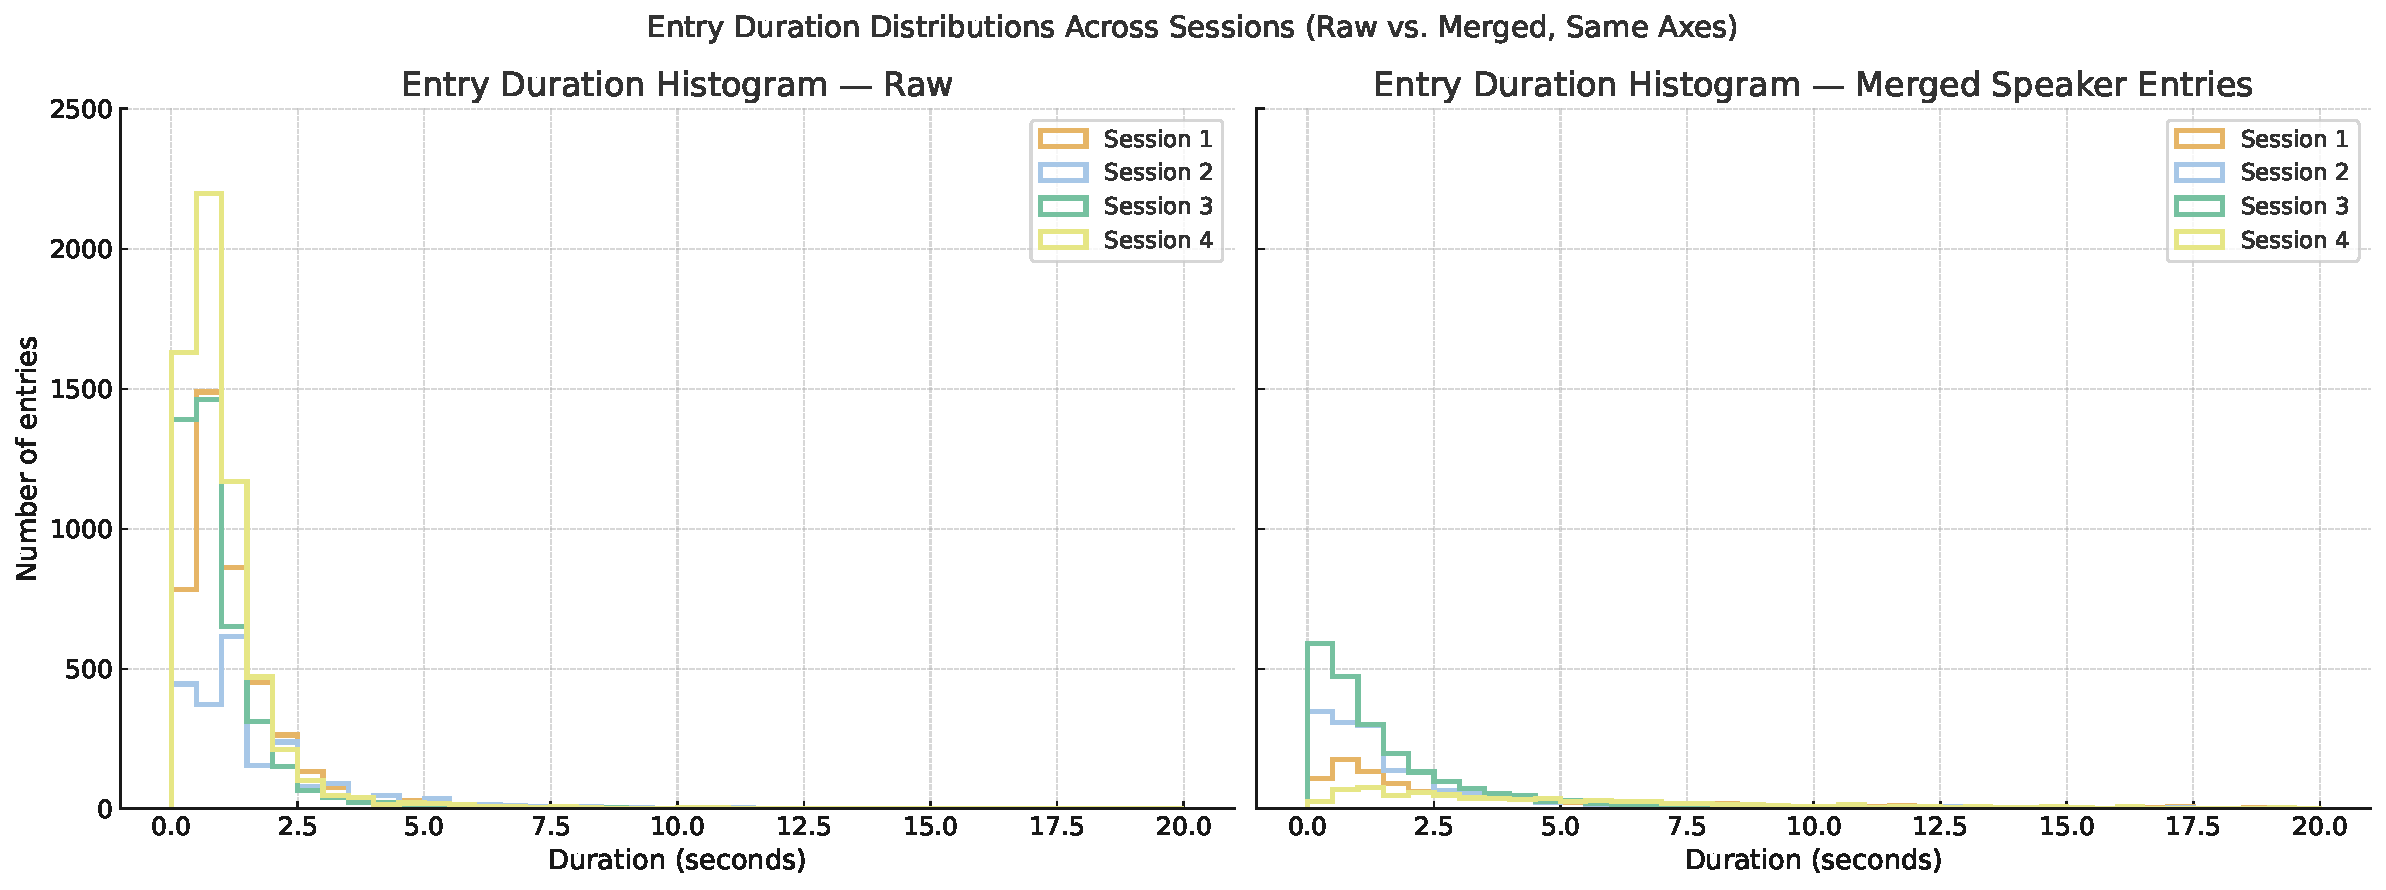
\includegraphics[width=\textwidth]{images/entry_duration_histograms_raw_vs_merged.pdf}
    \caption{Entry duration distributions across all four sessions, comparing raw transcripts (left) with merged speaker entries (right).}
    \label{fig:entry_duration_raw_merged}
\end{figure}

\begin{figure}[p]
    \centering
    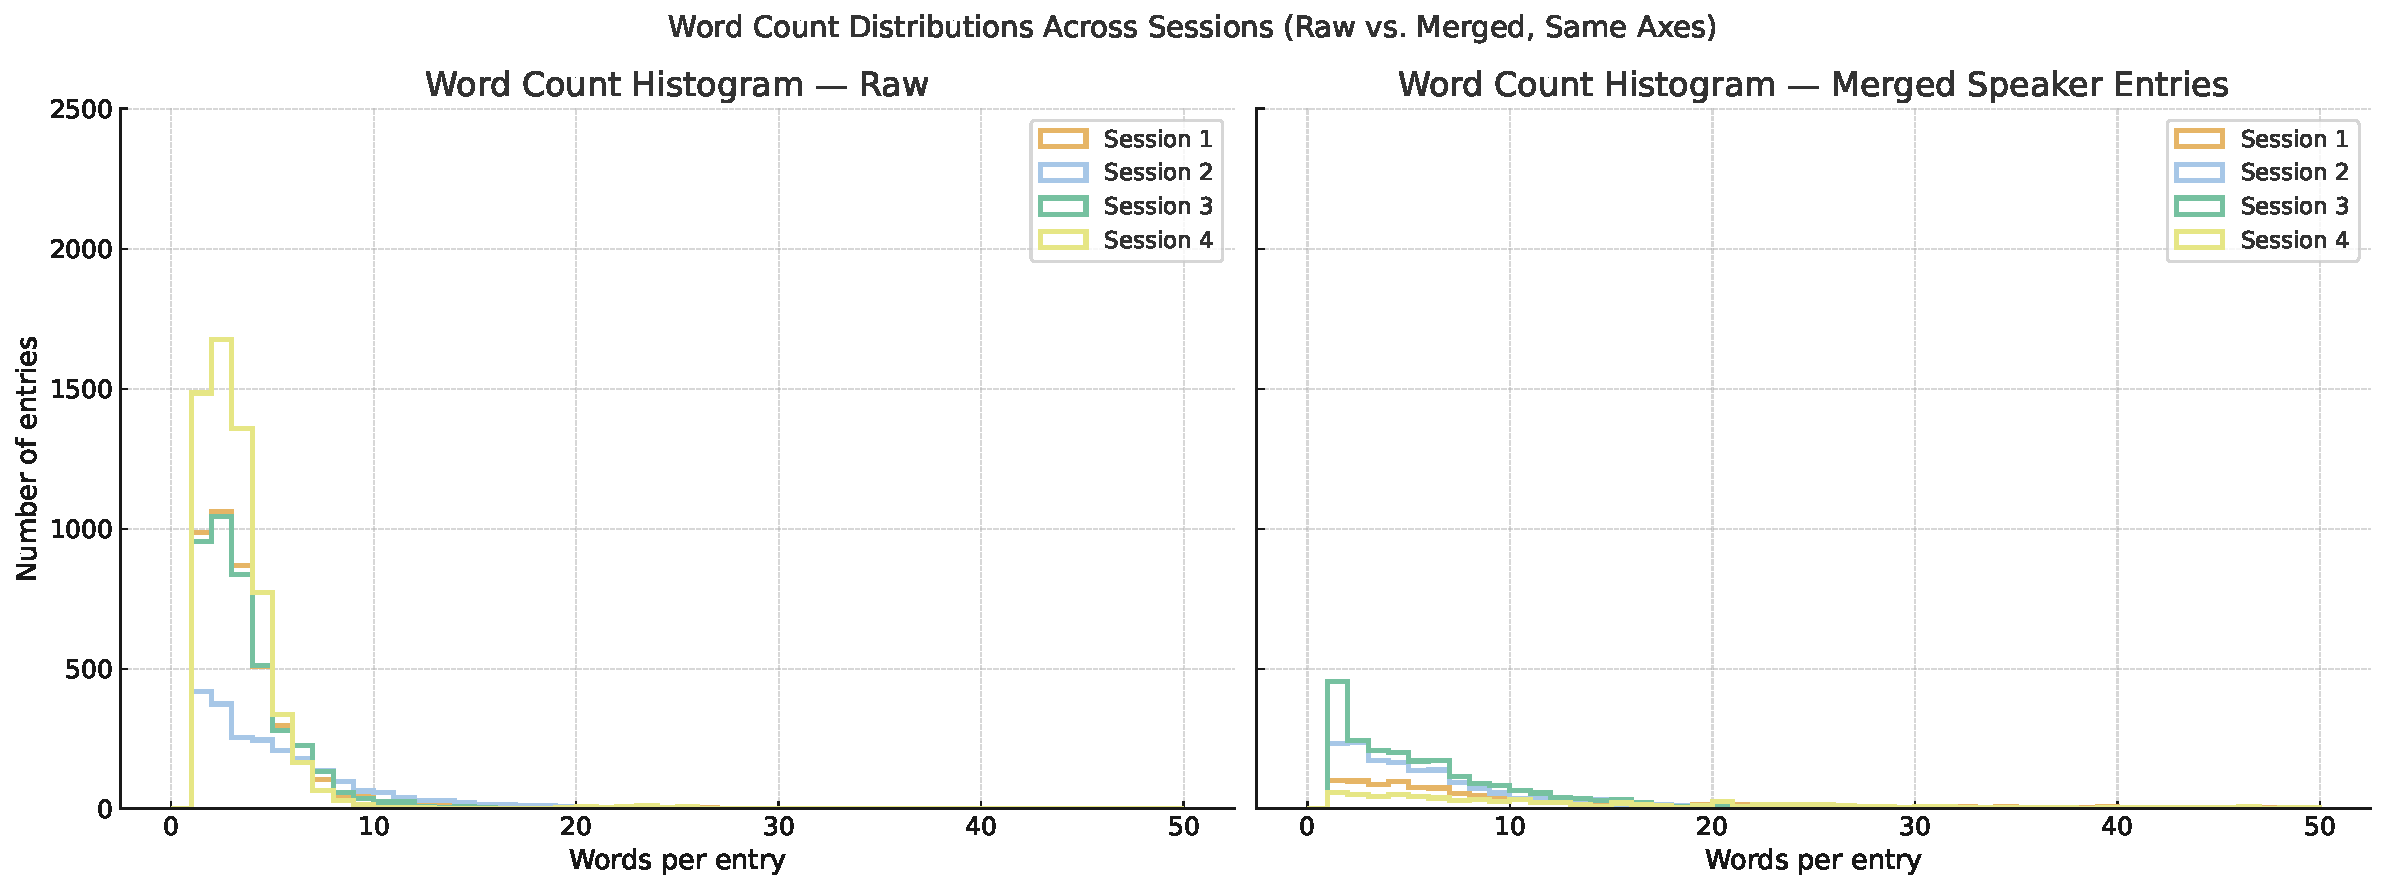
\includegraphics[width=\textwidth]{images/wordcount_histograms_raw_vs_merged.pdf}
    \caption{Word count distributions across all four sessions, comparing raw transcripts (left) with merged speaker entries (right).}
    \label{fig:wordcount_raw_merged}
\end{figure}

\begin{figure}[p]
    \centering
    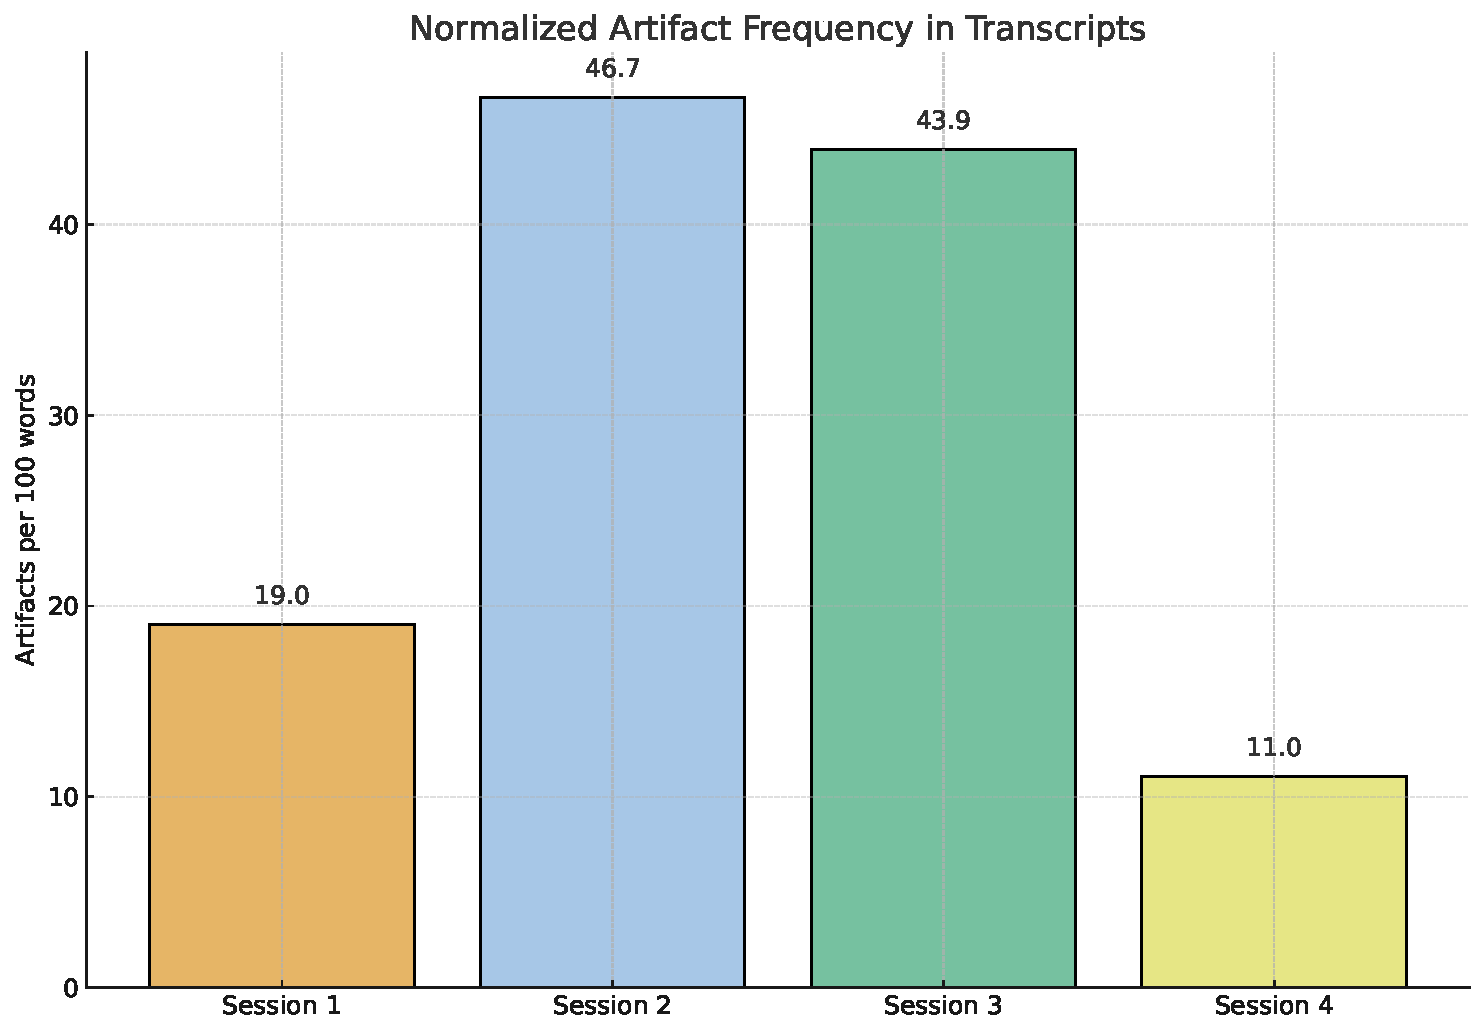
\includegraphics[width=0.9\textwidth]{images/normalized_artifact_frequency_sessions_colors.pdf}
    \caption{Normalized artifact frequency in transcripts, showing artifacts per 100 words for each session.}
    \label{fig:normalized_artifacts}
\end{figure}

\begin{figure}[p]
    \centering
    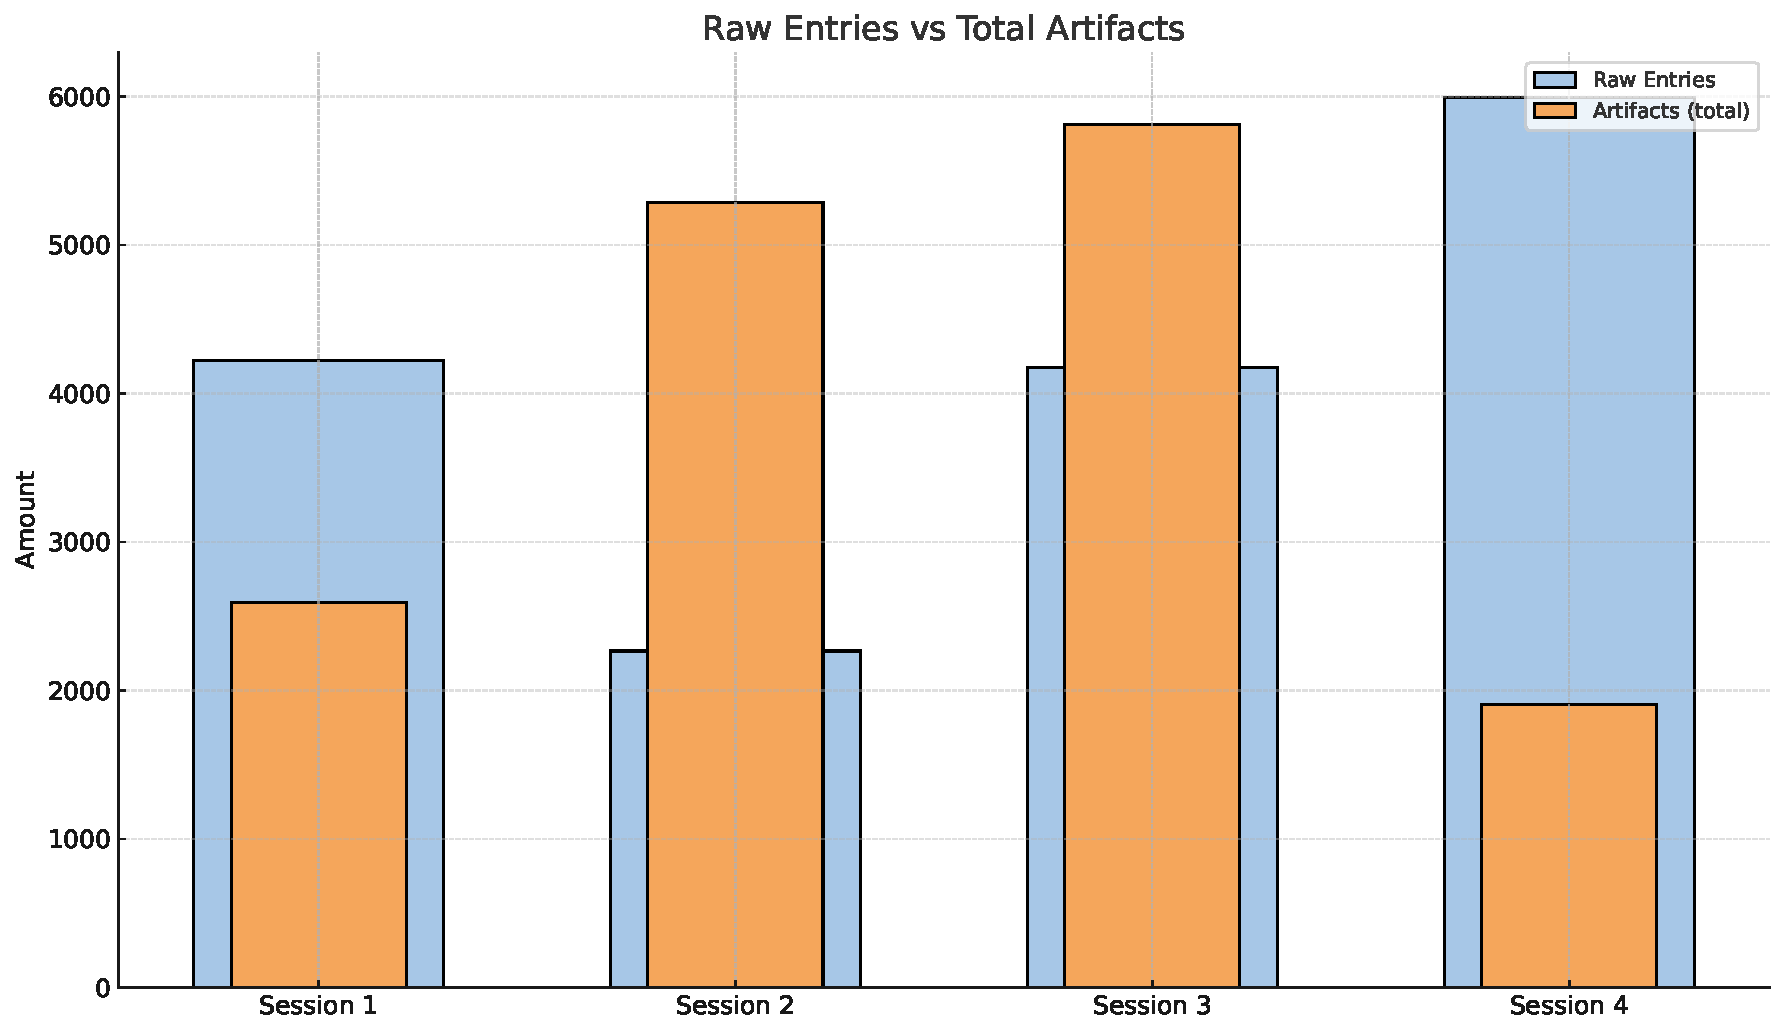
\includegraphics[width=0.9\textwidth]{images/raw_entries_vs_total_artifacts.pdf}
    \caption{Comparison between raw transcript entries and the number of detected artifacts per session.}
    \label{fig:raw_vs_artifacts}
\end{figure}

\begin{figure}[p]
    \centering
    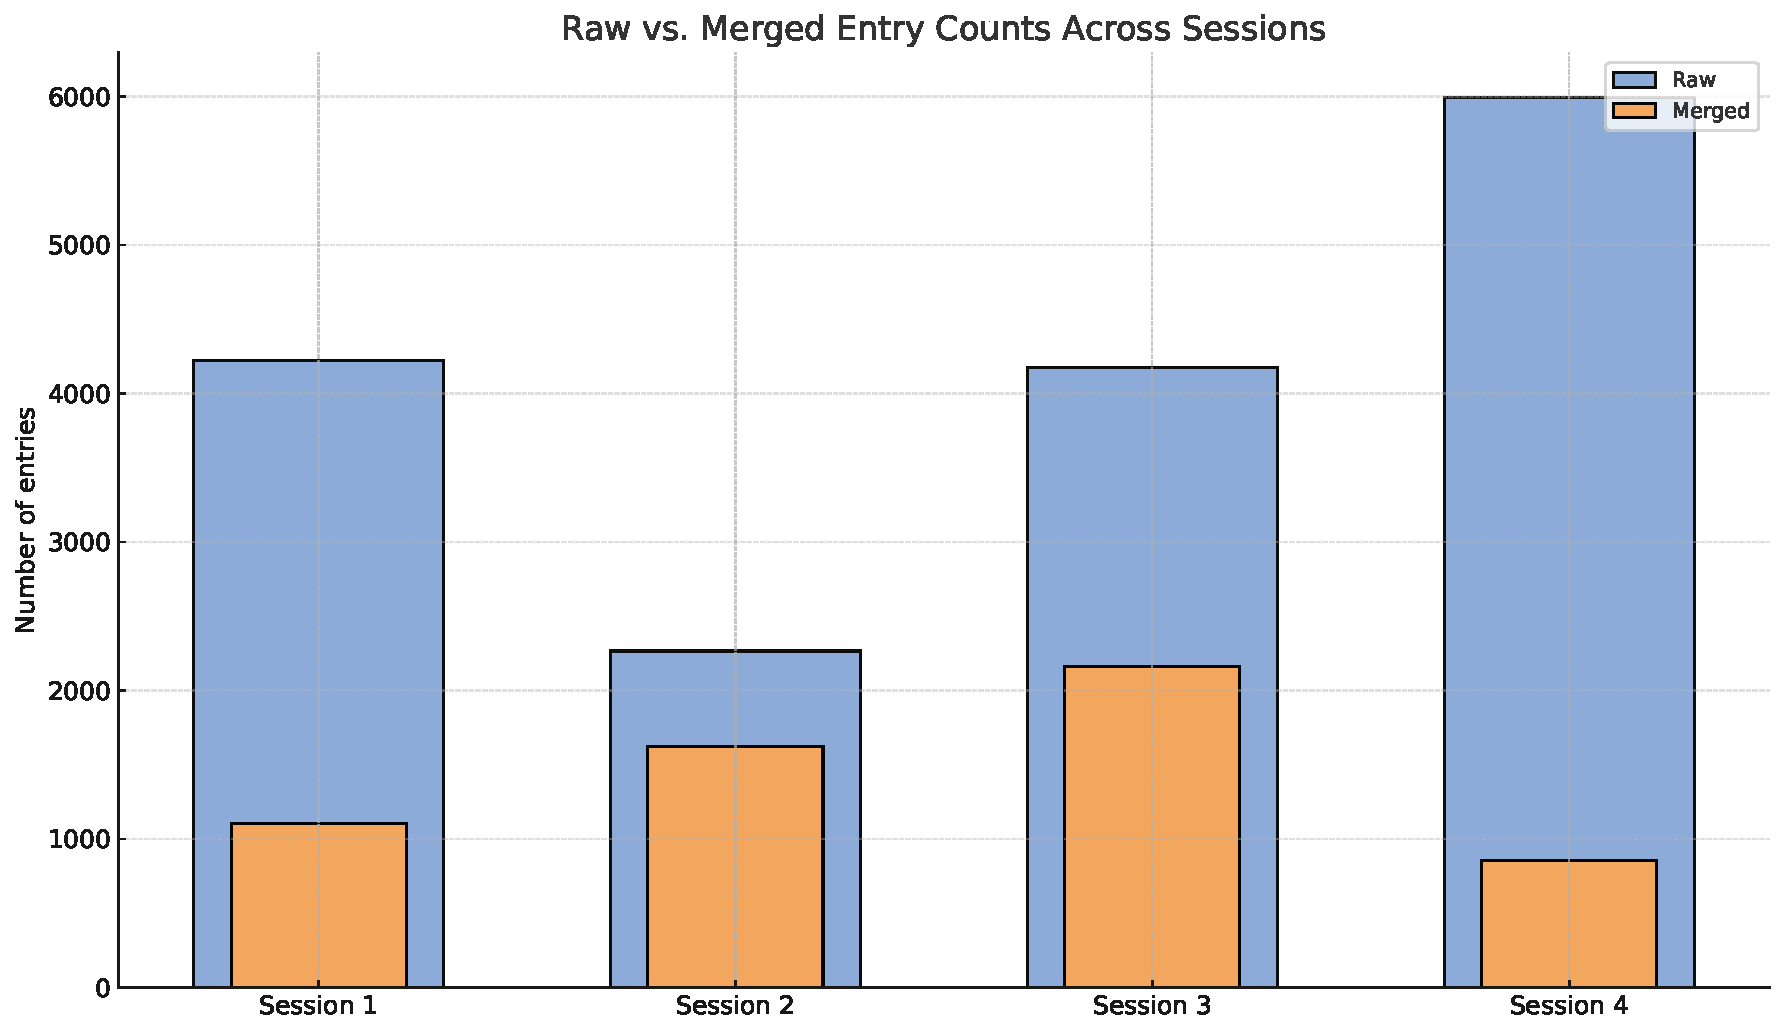
\includegraphics[width=0.9\textwidth]{images/raw_vs_merged_entry_counts.pdf}
    \caption{Number of transcript entries per session before and after merging consecutive same-speaker segments.}
    \label{fig:raw_vs_merged}
\end{figure}

\begin{figure}[p]
    \centering
    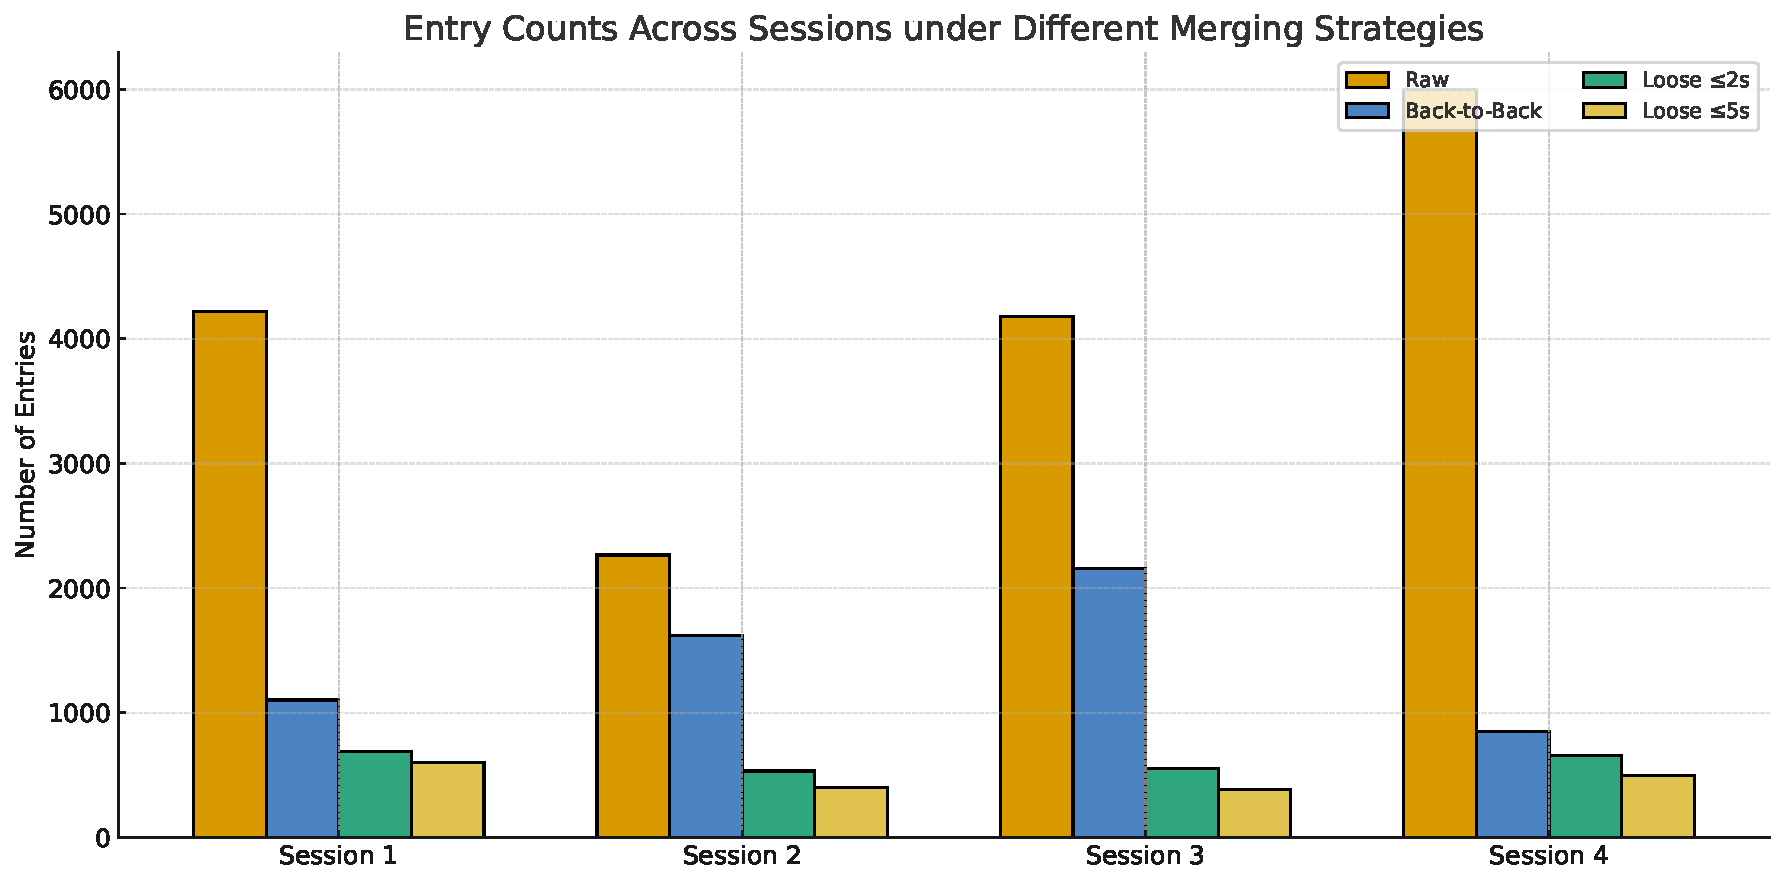
\includegraphics[width=0.9\textwidth]{images/entry_counts_across_sessions_merge_strategies.pdf}
    \caption{Entry counts across sessions under different merging strategies. Bars show the number of transcript entries per session when using raw data, simple back-to-back merging, and looser merges with 2s and 5s thresholds.}
    \label{fig:entry_counts_merge_strategies}
\end{figure}

\begin{figure}[p]
    \centering
    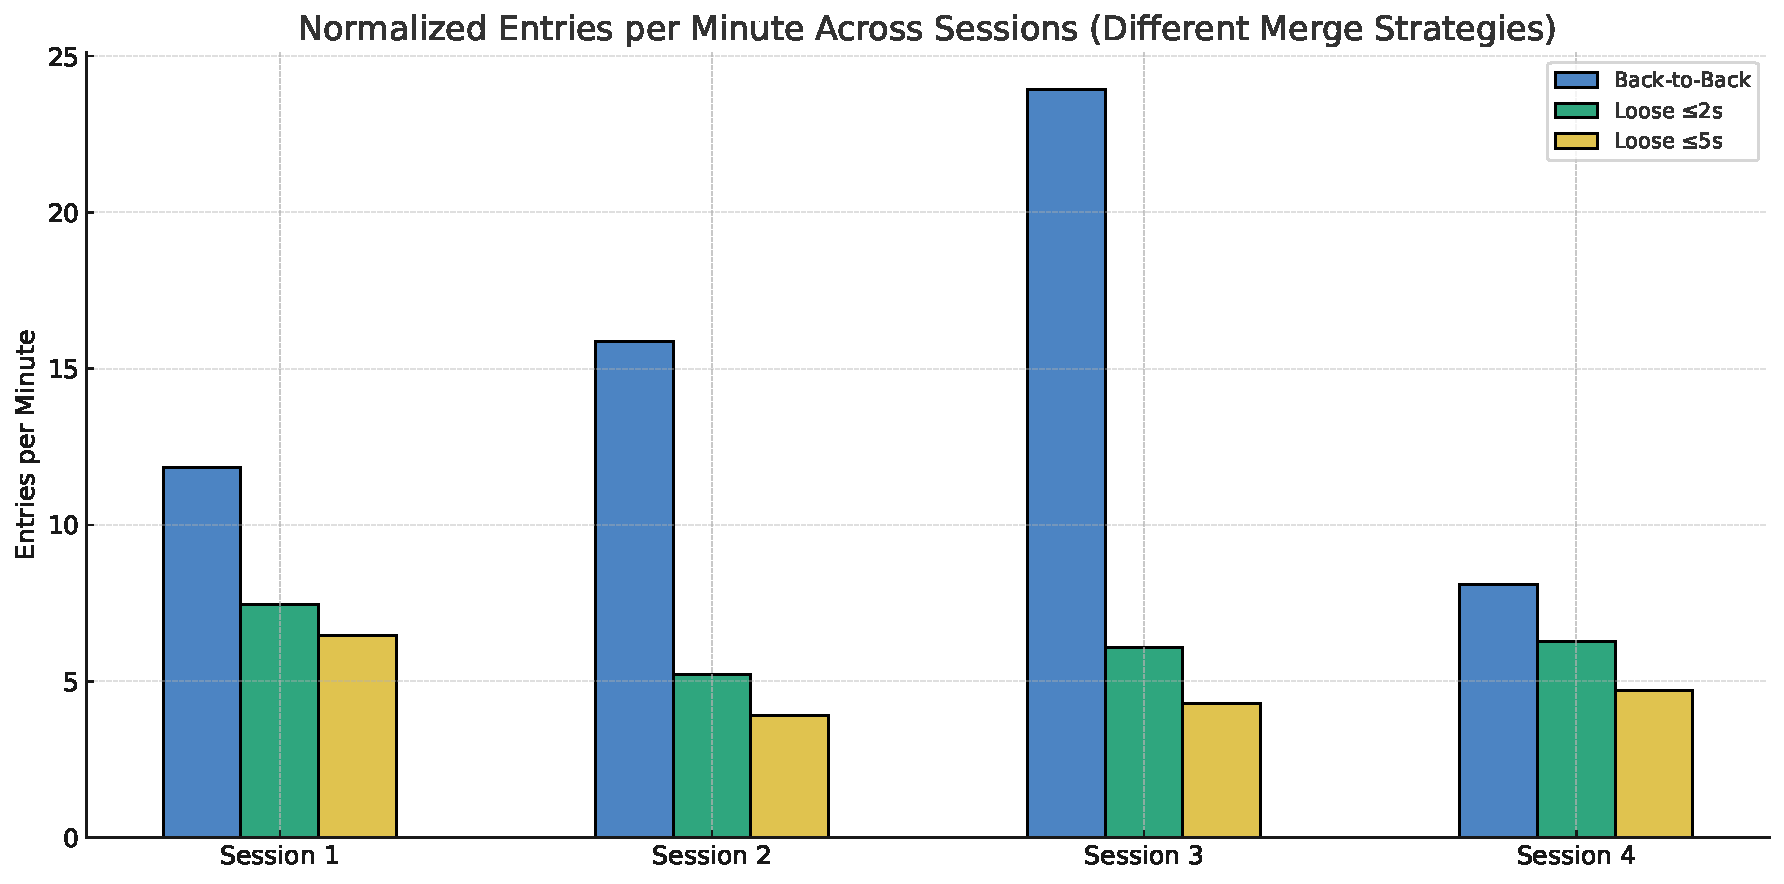
\includegraphics[width=0.9\textwidth]{images/normalized_entries_per_minute_merge_strategies.pdf}
    \caption{Normalized entries per minute across sessions for different merging strategies. Entries are adjusted by total session duration to allow fair comparison.}
    \label{fig:normalized_entries_merge_strategies}
\end{figure}

\begin{figure}[p]
    \centering
    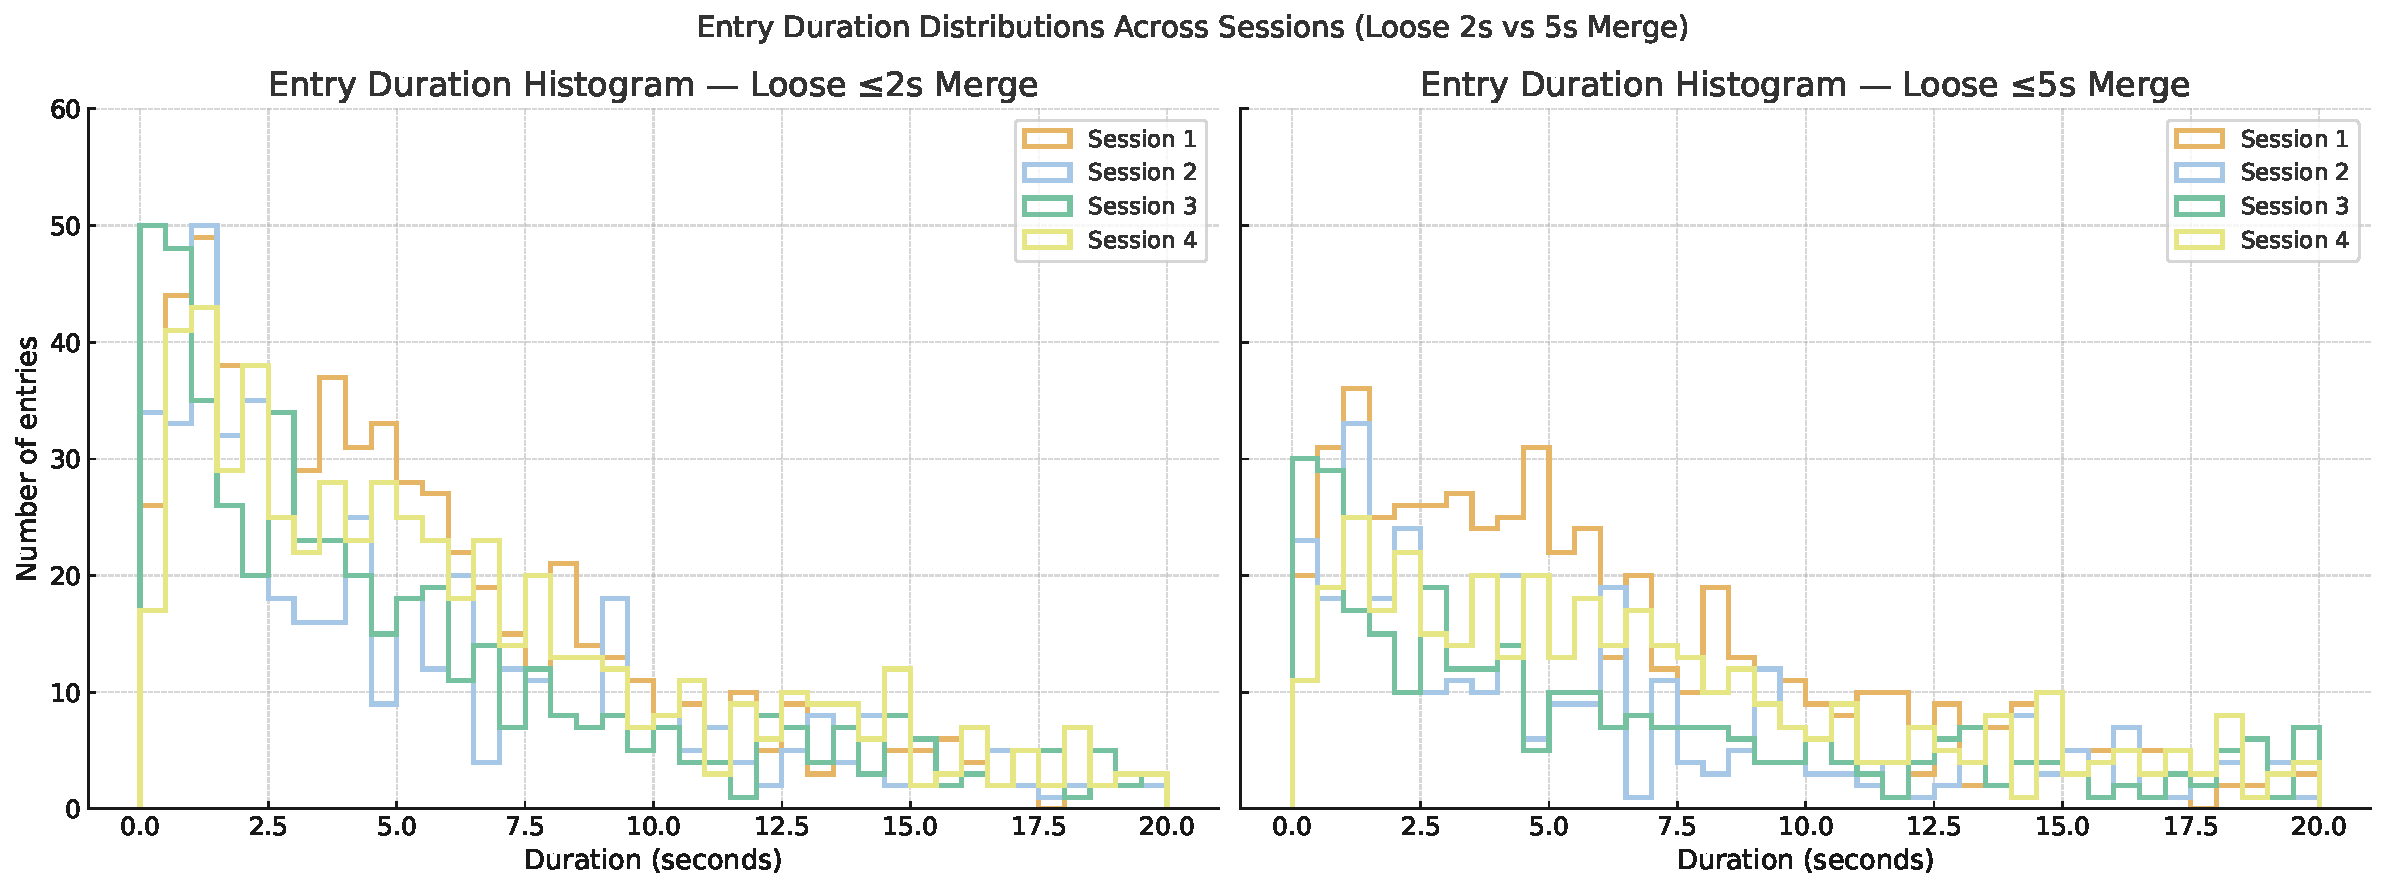
\includegraphics[width=\textwidth]{images/entry_duration_loose_merge.pdf}
    \caption{Entry duration distributions across all four sessions after time-based merging. Left: loose 2-second merge, Right: loose 5-second merge.}
    \label{fig:entry_duration_loose}
\end{figure}

\begin{figure}[p]
    \centering
    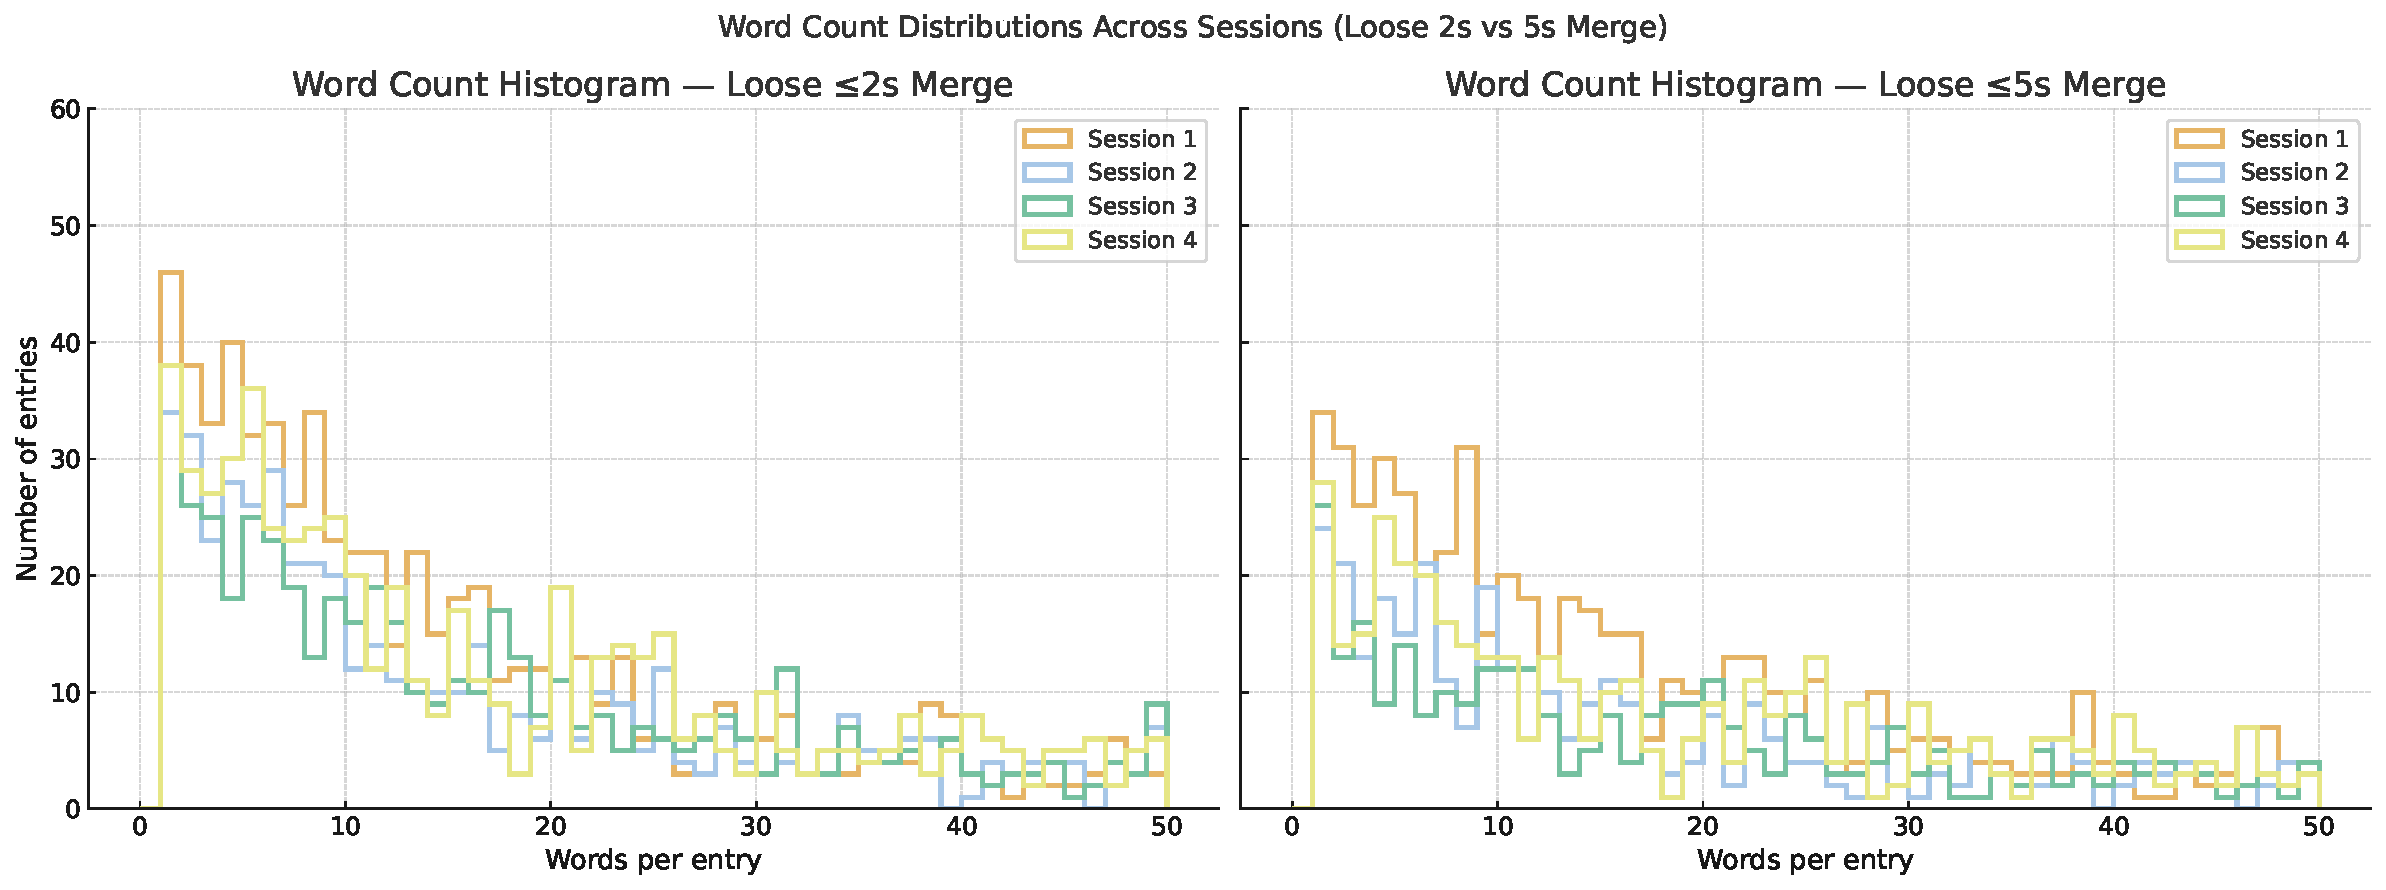
\includegraphics[width=\textwidth]{images/word_count_loose_merge.pdf}
    \caption{Word count distributions across all four sessions after time-based merging. Left: loose 2-second merge, Right: loose 5-second merge.}
    \label{fig:wordcount_loose}
\end{figure}

\clearpage


\begin{figure}[p] % 'p' puts it on a float-only page
  \centering

  % --- Word Count ---
  \begin{minipage}{0.45\linewidth}
    
\includegraphics[width=\linewidth]{fig_wordcount_raw.pdf}
    \caption*{(a) Word count (raw)}
  \end{minipage}\hfill
  \begin{minipage}{0.45\linewidth}
    
\includegraphics[width=\linewidth]{fig_wordcount_merged.pdf}
    \caption*{(b) Word count (merged)}
  \end{minipage}

  \vspace{1em}

  % --- Histogram of Durations ---
  \begin{minipage}{0.45\linewidth}
    
\includegraphics[width=\linewidth]{fig_duration_hist_raw.pdf}
    \caption*{(c) Durations (raw)}
  \end{minipage}\hfill
  \begin{minipage}{0.45\linewidth}
    
\includegraphics[width=\linewidth]{fig_duration_hist_merged.pdf}
    \caption*{(d) Durations (merged)}
  \end{minipage}

  \vspace{1em}

  % --- Scatter of Durations ---
  \begin{minipage}{0.45\linewidth}
    
\includegraphics[width=\linewidth]{fig_duration_scatter_raw.pdf}
    \caption*{(e) Scatter (raw)}
  \end{minipage}\hfill
  \begin{minipage}{0.45\linewidth}
    
\includegraphics[width=\linewidth]{fig_duration_scatter_merged.pdf}
    \caption*{(f) Scatter (merged)}
  \end{minipage}

  \caption{Comparison of raw and merged transcript statistics. Raw data shows extreme fragmentation, while merged data yields fewer, longer, and more coherent entries. All 6 graphs have been made with ChatGPT-5}
  \label{fig:raw-vs-merged}
\end{figure}

\subsection*{Script generation}
The second step in the pipeline.


\begin{itemize}
  \item \textbf{Dice / Rolls:} roll, rolled, rolling, dice, die, d20, d12, d10, d8, d6, d4, nat 20, nat 1, natural 20, natural 1
  \item \textbf{Checks \& Skills:} check, skill, saving throw, save
  \begin{itemize}
    \item acrobatics, animal handling, arcana, athletics, deception, history, insight, intimidation, investigation, medicine, nature, perception, performance, persuasion, religion, sleight of hand, stealth, survival
  \end{itemize}
  \item \textbf{Combat / Rules:} initiative, AC, armor class, hit points, HP, damage, dmg, critical, crit, advantage, disadvantage, rule, rules
\end{itemize}

\begin{table}[h]
\centering
\begin{tabular}{l r}
\hline
\textbf{Term} & \textbf{Occurrences in text entries} \\
\hline
damage & 5 \\
check & 4 \\
roll & 3 \\
medicine & 2 \\
survival & 1 \\
initiative & 1 \\
stealth & 1 \\
investigation & 1 \\
AC & 1 \\
hit points & 1 \\
\hline
\end{tabular}
\caption{Occurrences of mechanics-related terms in the \texttt{text} field of the comic book script dataset. Only terms with at least one match are shown.}
\label{tab:mechanics-leakage-text}
\end{table}



\begin{figure}[t]
  \centering
  
\includegraphics[width=\linewidth]{fig_duration_bins05_merged.pdf}
  \caption{Word count distribution of raw transcript entries. Most entries contain only 1-3 words, indicating heavy fragmentation.}
  \label{fig:wordcount-raw}
\end{figure}

\section{Expert review}

\section{The minimal viable product}
The minimal viable product (MVP) is a version of a new product that includes only the essential features necessary to meet the needs for initial testing. The goal of an MVP is to validate the product idea with minimal resources and gather feedback for future development. In figure \ref{fig:MVP} you can see the result of the MVP and in figure \ref{fig:MVPpipeline} you can see the pipeline that is used for the MVP.

\begin{figure}[!htp]
    \centering
    \includegraphics[scale=0.1]{images/mvpTTRPGtoComic.png}
    \caption[The minimal viable product]{The minimal viable product}
    \label{fig:MVP}
\end{figure}



\subsection{The minimal viable product}

\section{Small experiments}

\subsection{The language of TTRPGs}
Models like Whisper are trained on a wide variety of audio data, however this is primarily normal language usage. Because of this I anticipate that there will be a large issue with transcribing many fantasy words and terms, thus a small experiment has been done to identify if this is truly a problem. For this experiment 10 fantasy creature names have been recorded and whisper transcribed these 10 names. Only 1 out of the 10 names were transcribed correctly and 2 out of 10 where almost correct \ref{tab:monster_names}. This is inaccuracy is a big issue when transcribing any fantasy game session as it will interfere with many important key moments and key names during a session/campaign. When the group meets a monster called a "Slaad" and Whisper transcribes this as "Nod" it will quite confusing to understand what is going on in the story.

To generate a accurate transcription of the names a custom model needs to be trained on specific fantasy words and terms, however this is way outside of the scope of this thesis. In addition it is also very difficult as Fantasy names are fantasy names for a reason and people can just come up with new names all the time. Integrating thousands of names however could still be valuable as it will most likely catch most cases.
\begin{table}[h!]
\centering
\begin{tabular}{|l|l|}
\hline
\textbf{Correct Name} & \textbf{Transcribed name} \\
\hline
Owlbear    & Halber     \\
Goblin     & Goblin     \\
Rakshasa   & Raksasa    \\
Dracolich  & Draco Lich \\
Quasit     & Kwasi      \\
Slaad      & Nod        \\
Drow       & Drought    \\
Illithid   & Illidan    \\
Cambion    & Kempion    \\
Ankheg     & Hank Man   \\
\hline
\end{tabular}
\caption{Comparison of monster names and whisper transcribed versions}
\label{tab:monster_names}
\end{table}

\section{Generating the comic book script}
The iterative design process of generating the comic book script after the MVP version was a crucial step to improve the quality of the comic book panels. From having a one-shot approach where we gave the entire transcript to the LLama 3.1 model, we moved to an adaptive panel generator which has a structured approach to data and keeps track of the context. In this section all the iterative steps are described and what did and did not work in chronological order.

\subsubsection{MVP}
For the MVP of the artefact the entire transcript of the tabletop role-playing game session was given to Llama 3.1 and see what it would generate. The LLM was asked: "You are given a Dungeons and Dragons session transcript. Convert it into a comic book script." This resulted in two results: The LLM crashed as the token limit was exceeded or it gave things that had nothing to do to with the input and hallucinated everything. A quick fix to this was to cut the transcript into smaller chunks of text which resulted in an interesting result as it actually gave a comic book script. It was given 2 scenes of text which where hand cut out of the transcript. However as the LLM was not instructed to give a structured output it was useless as every time the program was run it would give a different output. The last step was to create a structured prompt for the LLM which is the prompt in \ref{lst:MPVLlamaprompt}. This resulted in a consistent JSON format output which could then be used to generate images.

\subsubsection{Cleaning up the transcript}
When you feed an audio recording to Whisper it transcribes the audio as one long sentence. There is no punctation or any idea of sentences structure. This way it is impossible to keep track of who said what and when. To fix this the transcript needs to be cleaned up. The first step is to use a Punctuation and Capitalization Restoration model \cite{guhrEtAl} to add punctuation and capitalization to the text. This will make the text more readable and easier to understand for an LLM. The second step is to use Speaker Diarization to identify the different speakers in the text. The tool used to do this was pyannote 3.1 \cite{Bredin23,Plaquet23}, an open source python library which is super easy to use and broadly used by people (15 million download per month). Lastly combine the cleaned up whisper transcription with the speaker diarization to create a structured JSON file. This new transcript file \ref{lst:sessionTrarnscriptJSON} is what created the foundation for the entire comic book generator.

\begin{lstlisting}[style=jsonstyle, caption={Session transcript JSON}, label={lst:sessionTrarnscriptJSON}]
{
    "panel_index": 0,
    "speaker": "SPEAKER_02",
    "text": "Our story actually starts with the three of you...",
    "start": 0.0,
    "end": 2.96
},
...
\end{lstlisting}

\subsubsection{Scene detection}

\subsubsection{Line based chunking}
Every line or every X lines

\subsubsection{LLM based chunking}
Scene cutting

\subsubsection{LLM based filtering}
Ask the LLM to decide if a line of text is player or character speech. Into giving it a chunk instead.

\subsubsection{Context aware LLM based chunking}

\subsubsection{Adaptive panel generating}

\section{Experimental setup}
To test the system on tool functionality, but primarily to test for the design requirements of a retelling system 3 different TTRPG sessions have been recorded and converted to a comic book. These comic books where then handed to the players and feedback was acquired using the INSERTHERE questionnaire. The comic books have also been cross-referenced with each other and with the original recording to see if there are differences in the generated comic book, but which are the same in the sessions.
\subsubsection{Experimental sessions}
One Dungeons and Dragon 5th edition dungeon master hosted 3 sessions with 2 or 3 players. Each session was the same scenario and lasted 1 to 2 hours. This setup was chosen as this makes the experiment as consistent as possible, but with important possible deviations.

Dungeons and Dragons 5th Edition was chosen as the TTRPG of choise, because there is easy access to many people with a lot of playing experience of this game. It is one of, if the the largest, TTRPG game that is currently being played. It is important to have a game which people know how to play, because I want to minimise the rule based conversations in the recording as much as possible. Rule conversations are an extra dimension of complexity for the system and this should be avoided as much as possible.

\subsubsection{}


\subsubsection{Participent feedback}
Participent have been asked feedback based on a customized version of the INSERTHERE questionaire. 

\subsection{Analyzing the generated comic books}
